\documentclass[11pt,a4paper,oneside,oldfontcommands]{ctexart}
\usepackage{tabularx}
\usepackage{array}
\usepackage{bm}
\usepackage{hyperref}
\usepackage{graphicx} 
\usepackage{amsmath}
\usepackage{algorithm}
\usepackage{algpseudocode}
\usepackage{fancyhdr}
\pagestyle{fancy}
\usepackage{color}
\usepackage{xcolor}
\definecolor{keywordcolor}{rgb}{0.8,0.1,0.5}
\usepackage{listings}


\definecolor{mygreen}{rgb}{0,0.6,0}  
\definecolor{mygray}{rgb}{0.5,0.5,0.5}  
\definecolor{mymauve}{rgb}{0.58,0,0.82}  
  
\lstset{ %  
  backgroundcolor=\color{white},   % choose the background color; you must add \usepackage{color} or \usepackage{xcolor}  
  basicstyle=\footnotesize,        % the size of the fonts that are used for the code  
  breakatwhitespace=false,         % sets if automatic breaks should only happen at whitespace  
  breaklines=true,                 % sets automatic line breaking  
  captionpos=bl,                    % sets the caption-position to bottom  
  commentstyle=\color{mygreen},    % comment style  
  deletekeywords={...},            % if you want to delete keywords from the given language  
  escapeinside={\%*}{*)},          % if you want to add LaTeX within your code  
  extendedchars=true,              % lets you use non-ASCII characters; for 8-bits encodings only, does not work with UTF-8  
  frame=single,                    % adds a frame around the code  
  keepspaces=true,                 % keeps spaces in text, useful for keeping indentation of code (possibly needs columns=flexible)  
  keywordstyle=\color{blue},       % keyword style  
  %language=Python,                 % the language of the code  
  morekeywords={*,...},            % if you want to add more keywords to the set  
  numbers=left,                    % where to put the line-numbers; possible values are (none, left, right)  
  numbersep=5pt,                   % how far the line-numbers are from the code  
  numberstyle=\tiny\color{mygray}, % the style that is used for the line-numbers  
  rulecolor=\color{black},         % if not set, the frame-color may be changed on line-breaks within not-black text (e.g. comments (green here))  
  showspaces=false,                % show spaces everywhere adding particular underscores; it overrides 'showstringspaces'  
  showstringspaces=false,          % underline spaces within strings only  
  showtabs=false,                  % show tabs within strings adding particular underscores  
  stepnumber=1,                    % the step between two line-numbers. If it's 1, each line will be numbered  
  stringstyle=\color{orange},     % string literal style  
  tabsize=2,                       % sets default tabsize to 2 spaces  
  %title=myPython.py                   % show the filename of files included with \lstinputlisting; also try caption instead of title  
}  
\hypersetup{hypertex=true,
	colorlinks=true,
	linkcolor=red,
	anchorcolor=blue,
	citecolor=blue}
\fancyhf{}
\chead{\textbf{算法设计与分析}}
\fancyhead[r]{\bfseries\thepage}
\fancyhead[l]{\bfseries\rightmark}
\renewcommand{\headrulewidth}{0.4pt} % 注意不用 \setlength
\renewcommand{\footrulewidth}{0pt}

\floatname{algorithm}{算法}
\renewcommand{\algorithmicrequire}{\textbf{输入:}}
\renewcommand{\algorithmicensure}{\textbf{输出:}}

\begin{titlepage}
	\title{\Huge\textbf{算法设计与分析 作业五}\\}
	\author{\Large\textbf{作者}:吴润泽 \and{\Large\textbf{学号}:181860109}\\
	\\
	\and {\Large\textbf{Email}:\href{mailto:181860109@smail.nju.edu.cn}{181860109@smail.nju.edu.cn}}\\}
	\date{\Large\today}
\end{titlepage}
\begin{document}
\maketitle
\newpage
\tableofcontents
\cleardoublepage
\section*{Chapter 10}
\markright{Chapter 10}
\addcontentsline{toc}{section}{Chapter 10}
{\subsection*{problem 10.3}}
\markright{problem 10.3}
\addcontentsline{toc}{subsection}{problem 10.3}
起始时刻将$v_1$加入队列中,在第一次循环中将其弹出,
$v_1$与n-1个点均有边相连,故将n-1条边及其权值加入队列。
在第二次循环时,需要将n-1条边中权值最小的边弹出,故需要比较n-2次。
{\subsection*{problem 10.4}}
\markright{problem 10.4}
\addcontentsline{toc}{subsection}{problem 10.4}
\paragraph*{1)}
起始n-1条边,比较n-2次;\\
第二次2(n-2)条边,比较2n-5次;\\
...因此共需要$\sum\limits_{i=1}^{n-1}(n-i)i-1=\frac{1}{6}(n^3-7n+6)$次比较。
\paragraph*{2)}
起始时刻将$v_1$加入队列中,在第一次循环中将其弹出,
$v_1$与n-1个点均有边相连,故将n-1条边及其权值加入队列。而队列存放的是节点的最小权值信息,最多为n-1个。
因此此时优先队列存在最多,最多n-1个节点。
{\subsection*{problem 10.8}}
\markright{problem 10.8}
\addcontentsline{toc}{subsection}{problem 10.8}
\paragraph*{1)}
最大生成树与最小生成树的本质是相同的,将prim算法中维护权值最小的队列改为维护权值最大的队列即可。
\begin{lstlisting}[language=C++,title=PrimBig.func]
PrimBig(G):
	initialize all nodes in G as UNSEEN
	initialize the priority queue queNode as empty
	initialize edge set MST as empty /*存放当前局部最大生成树中的边*/
	Select an arbitrary vertex s to start building the maximum spanning tree
	s.candidateEdge:=NULL 
	/*每个顶点的candidateEdge,标记它是通过哪条边被连入最大生成树*/
	queNode.INSERT(s,MAX) /*起始点s的权值设为最高,必然先被调度执行*/
	while queNode!=empty:
		v:=queNode.EXTRACT-MAX() /*每次选取队列中权值最大的边*/
		MST:=MST.add{v.candidateEdge} /*将该边加入最大生成树*/
		UPDATE-FRINGE(v,queNode)
	return MST
UPDATE-FRINGE(v,queNode):
	for neighbor w of v:
		newWeight:=vw.weight
		if w is UNSEEN: /*如果是第一次遍历到*/
			Fringe.INSERT(w,newWeight)  /*将w加入队列*/
		else:
			if newWeight>w.priority:
				w.candidateEdge:=vw
				Fringe.decrease(w,newWeight) /*将w的权值更新为较大的边权*/
\end{lstlisting}
\paragraph*{2)}
对于最大生成树T,未被选取的边中,任意选择一条加入T中,必定成环,且为环中权值最小的边。
即最大生成树未被选择的边即为最小的反馈边集。因此最大生成树算法结束后,遍历所有边记录未被选择的即可。
遍历仅需线性时间,最大生成树算法采用优先队列时间复杂度$O((m+n)\log n)$。
\begin{lstlisting}[language=C++,title=PrimFES.func]
PrimFES(G):
	MST:=PrimBig(G)
	return G(E)-MST /*将E中MST抛去剩下的便是FES*/
\end{lstlisting}
{\subsection*{problem 10.9}}
\markright{problem 10.9}
\addcontentsline{toc}{subsection}{problem 10.9}
\paragraph*{不可能}以结点s为起点,使用Prim算法构造最小生成树,使用Dijkstra算法
构造单源最短路。两算法的第一次扩充都是选择s相邻结点中边权最小的边。
如果在相邻边中的最小边权唯一,则两者选择的边一定相同。\\
\hspace*{20pt}否则假设存在SU和SV两边权均为最小边权,
第一次循环中,Prim算法选择了SU,而Dijkstra算法选择了SV。
假设Dijkstra的结果没有选择SU,同时因为S与U有边相连,即S到达U的路径存在,
那么一定是通过V或者其他与S相邻的结点间接到达U,而边权值为正,即间接到达U的路径一定大于SU本身边权。
\\\hspace*{20pt}产生矛盾,故Dijkstra一定选择SU,与Prim算法有公共边SU。
\newpage
{\subsection*{problem 10.11}}
\markright{problem 10.11}
\addcontentsline{toc}{subsection}{problem 10.11}
\paragraph*{算法设计}
仿照Prim算法,对于循环中选择的边uv,
若$v\in U$则不能再以v为起点更新优先队列,即v只能以某一分支的终点出现。
即保证与U中结点有关的边只在T中出现一次。
如果循环结束时,选择的边数不足n-1说明不存在最轻生成树。
\paragraph*{时间复杂度}
判断是否在U中,可以采用布尔数组的方式,$O(1)$复杂度。
整体时间复杂度与Prim算法相同,采用优先队列的实现方式,时间复杂度为$O((m+n)\log n)$。
\begin{lstlisting}[language=C++,title=PrimMLT.func]
PrimMLT(G,U):
	/*初始化操作*/
	选择不在U中的点s作为Prim起点
	vis:=[] /*维护U中结点被访问的情况*/
	s.candidateEdge:=NULL
	/*每个顶点的candidateEdge,标记它是通过哪条边被连入生成树*/
	queNode.INSERT(s,MIN)
	while queNode!=empty:
		v:=queNode.EXTRACT-MIN()
		MLT:=MLT.add{v.candidateEdge} /*将该边加入生成树*/
		if MLT.size=n-1:return true
		if v not in U: /*在U中的点只能被用来作为边的终点*/
			UPDATE-FRINGE(v,queNode)
	return true
UPDATE-FRINGE(v,queNode):
	for neighbor w of v:
		newWeight:=vw.weight
		if w is UNSEEN: /*如果是第一次遍历到*/
			Fringe.INSERT(w,newWeight)  /*将w加入队列*/
		else if newWeight>w.priority:
				w.candidateEdge:=vw
				Fringe.decrease(w,newWeight) /*更新为较小权值*/
\end{lstlisting}
\newpage
{\subsection*{problem 10.13}}
\markright{problem 10.13}
\addcontentsline{toc}{subsection}{problem 10.13}
仿照Kruskal算法,在算法执行前进行预处理,将S中所有边加入MST并更新并查集,
并在剩余边中排序生成优先队列,进行Kruskal算法地执行。
\begin{lstlisting}[language=C++,title=KruskalNew.func]
KruskalNew(G,U):
	/*初始化操作*/
	initialize the tree MST to S /*将MST初始化为S*/
	initialize the disjoint  with S /*先将S中的边加入并查集*/
	while queNode!=empty:
		vw:=queNode.EXTRACT-MIN()
		if FIND(v)!=FIND(w):
			MST:=MST.add{vw} /*将该边加入生成树*/
			if MST.size=n-1: return /*已经找到n-1条边,则返回*/
			UNION(v,w) /*将两个并查集合并*/
\end{lstlisting}
{\subsection*{problem 10.15}}
\markright{problem 10.15}
\addcontentsline{toc}{subsection}{problem 10.15}
\paragraph*{1)}
错误,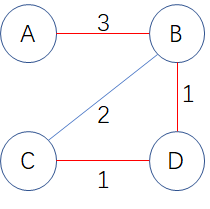
\includegraphics[height=100pt]{10-15-1.png}一定包含权值为2的唯一最重边。
\hypertarget{problem101502}{\paragraph*{2)}}
正确,假设vw是G的唯一最重边,在某个环内。如果vw是MCE,划分将v、w划分为两个部分,且v、w在环内,
则端点分别在两个集合的边不止一条,因为vw是MCE,则它不可能大于其余跨越集合的边的权重,与vw是唯一最重边矛盾。
因此vw一定不是MCE,而根据课本定理知,MST中的边一定为MCE,则vw不可能在任何一个MST中。
\paragraph*{3)}
正确,如果vw是图G唯一最轻边,采用Dijkstra算法,则第一步选择全局最小边一定选择vw。
如果vw不是唯一最轻边,假设不存在MST中含有vw,将vw加入任意一个MST中,则必然产生一个环路,
从环路中删去任意一条除了vw之外的边,形成的生成树权值和一定小于等于MST,与假设矛盾。因此vw必属于某个MST上。
\paragraph*{4)}
正确,与\textbf{3)}中第一种情况相同。
\paragraph*{5)}
错误,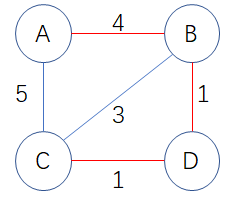
\includegraphics[height=100pt]{10-15-5.png},对于环ABC其上的BC边为唯一最轻边,但最小生成树中不含有边BC。
\paragraph*{6)}
错误,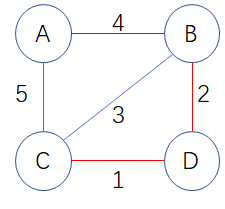
\includegraphics[height=100pt]{10-15-6.png},对于A和C两节点其最短路径为AC,但是图中的MST唯一且不包含AC。
\paragraph*{7)}
正确,对于Prim算法,对于边权只涉及到了大小的比较,与正负无关,对于含有负权边算法同样成立。
\hypertarget{problem1016}{\subsection*{problem 10.16}}
\markright{problem 10.16}
\addcontentsline{toc}{subsection}{problem 10.16}
\paragraph*{正确}{\textbf{引理 }}每条边权值不同的图的最小生成树唯一。\\
设G是所有边权均不相同的无向连通图,设T1,T2为G的两个MST,
取两MST不相同的边集中权值最小的边e,假设e在T2而不在T1中。
将e加入T1,则T1中产生一个包含e的环。如果e不是环中权值最大的边,则违背了最小生成树性质。
如果e是环中权值最大的边,由于环中不可能均为T2中的边,否咋T2将产生环,则取该环中不在T2的边v,
即v也处于两MST不相同的边集中,则v的权值小于e,与e是环中权值最大的边矛盾。
综上每条权值不同的图的最小生成树唯一。\\
原图和平方图中各边的大小顺序排列不变。
我们选取相同的起始点,对两个图执行Prim算法,每一轮选择的边均相同,
即T是G的最小生成树当且仅当T是G'的最小生成树。
{\subsection*{problem 10.18}}
\markright{problem 10.18}
\addcontentsline{toc}{subsection}{problem 10.18}
\paragraph*{1)}
\hyperlink{problem1016}{problem 10.16 引理}已证明。
\paragraph*{2)}
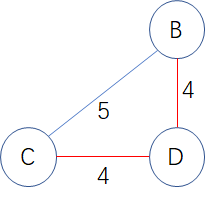
\includegraphics[height=100pt]{10-18-2.png}CD、BD边权相等,最小生成树即为红边所描。
\paragraph*{3)}
\textbf{不等价}
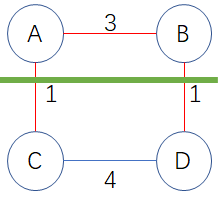
\includegraphics[height=100pt]{10-18.png}图中最小生成树为红边所连,
而将其划分为AB和CD各一组,跨越两个集合的最小权值边不唯一。
\paragraph*{4)}
\subsubsection*{算法设计}
\noindent1. 在进行Kruskal算法合并两个等价类时,
分别属于两个等价类的两个点的最长边一定是当前合并的边(权值按照递增顺序访问)。\\
2. xy不在MST中,加入MST中一定会成环,删去环上除xy以外权值最大的边,得到
当前树权值和。\\
3. 枚举所有不在MST中的边,得到最小的权值和与MST权值和比较,
判断是否相等。如果相等,说明存在不止一个MST。
\begin{lstlisting}[language=C++,title=SecMst.func]
SecMst(G(V,E)):
	mst:=GetMst(G) /*得到MST的权值和*/
	secmst:=0 /*记录其他生成树最小值*/
	for vw in E:
		if vw not in MST: /*枚举不在MST中的边*/
			secmst:=min(secmst,mst+weight(w)-path[v][w])
	if secmst=mst:return false /*MST不唯一*/
	else: return true /*MST唯一*/
GetMst(G(V,E)):
	/*初始化操作*/
	sum:=0 /*记录MST的权值和*/
	path:=[][] /*记录i j路径上的最长边*/
	while queNode!=empty:
		vw:=queNode.EXTRACT-MIN()
		if FIND(v)!=FIND(w):
			sum:=sum+weight(vw)
			MST:=MST.add{vw} /*将该边加入生成树*/
			for i in V:
				if FIND(i)!=FIND(v): continue
				for j in V:
					if FIND(j)!=FIND(v): continue
					path[i][j]:=path[j][i]:=weight(vw) 
					/*边权是递增的,最大值不断更新*/
			if MST.size=n-1: return sum /*已经找到n-1条边,则返回*/
			UNION(v,w) /*将两个并查集合并*/
\end{lstlisting}
{\subsection*{problem 10.19}}
\markright{problem 10.19}
\addcontentsline{toc}{subsection}{problem 10.19}
\paragraph*{1)}
假设有用边不在MST中,有用边e加到MST中,因为e不属于G中的任意环,
所以没有环路。此时有n条边,与MST性质矛盾。故假设不成立,即有用边在最小生成树中。
\paragraph*{2)}
由\hyperlink{problem101502}{problem 10.15 2)}可知,环路上的唯一最重边不可能成为MCE,
故不存在于任何MST中。
\paragraph*{3)}
\textbf{暴力算法}\\
\noindent 1. 将边权按照降序排列,复杂度$O(m\log m)$。\\
2. 依次遍历每条边,判断其是否为危险边,若是则将其删去。\\
2.1 判断vw是否为危险边,先删除vw,以w为起点进行DFS,记录搜索路径上的最大权,遇到v时DFS返回。
回溯路径上更新最大权值。
如果vw权值大于最大权值说明是这个环上的危险边,则删去,否则将vw加回。时间复杂度为$O(m(m+n))$。\\
3. 总的时间复杂度为$O(m(m+n))$。\\
\newpage
\begin{lstlisting}[language=C++,title=AntiKruskal.func]
AntiKruskal(G):
	降序排列所有边权值,结果存入edges
	for vw in edges:
		G.delete(vw) /*先删除vw,进行判断是否为危险边*/
		if vw.weight<DFSPath(w,v): /*即vw小于环路(或不是环路)的最大权边*/
			G.add(vw) /*不是危险边,将其加回*/
DFSPath(w,v):
	path:=0 /*DFS路径上的最大路径值*/
	w.color:=GRAY
	for neighbor u of w:
		if u.color=WHITE:
			if u=v /*遍历遇到v即环路则返回*/
				path:=wu.weight /*沿原路返回*/
				return path
			else:
				path:= max(wu.weight,DFS(u)) /*回溯后更新path最大值*/
	return path
\end{lstlisting}
\paragraph*{算法优化}
每次循环都要进行一次DFS遍历来判断是否为危险边,重复判断过多。
由\textbf{2)}可知,危险边(即不是MCE)一定不会被选做MST中的边,
同时由书中定理可知MCE一定被MST选择,并且权值各不相同,
由\hyperlink{problem1016}{problem 10.16 引理}MST唯一。因此MST未选择的边均为危险边。
则采用Kruskal算法生成MST,然后遍历所有边,未被选择的边即为危险边。时间复杂度为$O(m\log(m))$。
% 可以先将图中所有环找出,每次判断该边是否在环中,并且由于边权按照降序排列,首先出现的
{\subsection*{problem 10.21}}
\markright{problem 10.21}
\addcontentsline{toc}{subsection}{problem 10.21}
\paragraph*{不正确}
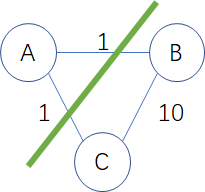
\includegraphics[height=100pt]{10-21.png}划分将A分为一组,BC分为一组,分别对两组进行最小生成树
,则BC边将被选择。两组间的割最小权为1,则产生的生成树权值和为11。而最小生成树选择AB和AC边,权值和为2。
\newpage
\section*{Chapter 11}
\markright{Chapter 11}
\addcontentsline{toc}{section}{Chapter 11}
{\subsection*{problem 11.1}}
\markright{problem 11.1}
\addcontentsline{toc}{subsection}{problem 11.1}
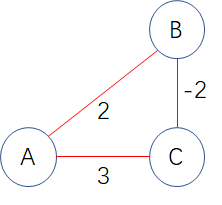
\includegraphics[height=100pt]{11-1.png}以A为起点,首先确定到达B的最短路径$A\rightarrow B$为2,
更新到达C最短长度为0,第二轮确定到C的最短路径为$A\rightarrow B\rightarrow C$为0。
而A到达B最短路径应为$A\rightarrow C\rightarrow B$为1,产生错误。
{\subsection*{problem 11.2}}
\markright{problem 11.2}
\addcontentsline{toc}{subsection}{problem 11.2}
\paragraph*{不一定}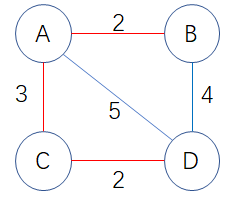
\includegraphics[height=100pt]{11-2.png},B到D的最短路径为BD,
而最小生成树(红边所示)不包含BD。
{\subsection*{problem 11.6}}
\markright{problem 11.6}
\addcontentsline{toc}{subsection}{problem 11.6}
\paragraph*{1)}
最小生成树不会变化。\\原图和边权加1后的图中各边的大小顺序排列不变。
我们选取相同的起始点,对两个图执行Prim算法,每一轮选择的边均相同,因此不会发生变化。
\paragraph*{2)}最短路径会发生变化。\\
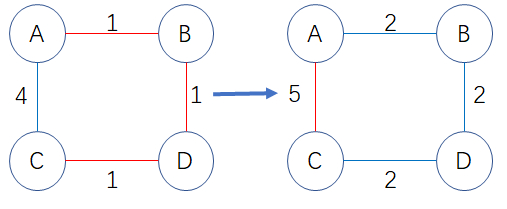
\includegraphics[height=100pt]{11-6.png}\\
AC的最短路径从$A\rightarrow B\rightarrow D\rightarrow C$边权为3,变为$A\rightarrow C$边权为5。
{\subsection*{problem 11.8}}
\markright{problem 11.8}
\addcontentsline{toc}{subsection}{problem 11.8}
仿照Dijkstra算法,将点权转化为边权,对于某一节点更新其邻居u的边权时,u的点权和边权放一起。
\begin{lstlisting}[language=C++,title=DijkstraPoint.func]
DijkstraPoint(G,s):
	/*初始化操作*/
	Cost:=[] /*所有节点的Cost初始化为0*/
	for neighbor w of s:
		queNode.INSERT(s,sw+point[s]) /*到达邻居节点的代价为边权加上s自身点权*/
	while queNode!=empty:
		v:=queNode.EXTRACT-MIN()
		Cost[v]:=v.priority /*记录v的最短路径权值*/
		UPDATE-FRINGE(v,queNode)
UPDATE-FRINGE(v,queNode):
	for neighbor w of v:
		newWeight:=v.priority+vw.weight+w.priority /*到达w的代价为到达v的代价加上vw边权和w点权*/
		if w is UNSEEN: /*如果是第一次遍历到*/
			Fringe.INSERT(w,newWeight)  /*将w加入队列*/
		else if newWeight>w.priority:
				w.candidateEdge:=vw
				Fringe.decrease(w,newWeight) /*更新为较小权值*/
\end{lstlisting}
{\subsection*{problem 11.9}}
\markright{problem 11.9}
\addcontentsline{toc}{subsection}{problem 11.9}
\noindent \textbf{适用 }
证循环不变式:当结点u被加入到集合S时,$u.d=\delta(s,u)$成立即可。\\

设结点u是第一个加入到集合S时是的该不变式不成立的结点,
即$u.d\neq\delta(s,u)$。由于结点s是第一个加入到集合S中的结点,并且$s.d=\delta(s,s)=0$,
结点u必定与s不同。集合S在将结点u加入之前为非空。此时一定存在某条从s到u的路径,否则
,$u.d=\delta(s,u)=\infty$,与$u.d\neq\delta(s,u)$产生矛盾。故存在一条从s到u的最短路径p。
设p为$s\rightarrow x\rightarrow y\rightarrow u,x\in S,y\in(V-S)$,\\

在结点x加入集合S时,边xy被松弛,则有$y.d=\delta(s,y)$。
因为y是结点s到u的一条最短路径上,除了s到达邻居节点的边权可能为负外其余节点为正值。
则$\delta(s,y)\leq\delta(s,u)$,即$y.d=\delta(s,y)\leq \delta(s,u)\leq u.d$。
但是u与y均在V-S里,选择了u则有$u.d\leq y.d$。因此$y.d=\delta(s,y)=\delta(s,u)=u.d$与假设矛盾。
因此不变式:当结点u被加入到集合S时,$u.d=\delta(s,u)$依旧成立。
{\subsection*{problem 11.10}}
\markright{problem 11.10}
\addcontentsline{toc}{subsection}{problem 11.10}
\paragraph*{1)}数学归纳法:\\
当n=1,2时,显然成立。\\
假设n=k时,存在一条哈密顿路径$v_1\rightarrow v_2\rightarrow \cdots \rightarrow v_k$。\\
当n=k+1时,\\
当$v_k\rightarrow v_{k+1}$时,存在哈密顿路径$v_1\rightarrow v_2\rightarrow \cdots \rightarrow v_k\rightarrow v_{k+1}$。\\
当$v_{k+1}\rightarrow v_{k}$时,则按照下标向前寻找,\\
如果存在$v_i\rightarrow v_{k+1},v_{k+1}\rightarrow v_{i+1}$,
\\则可构造哈密顿路径
$v_1\rightarrow v_2\rightarrow\cdots\rightarrow v_i\rightarrow v_{k+1} \rightarrow v_{i+1}\rightarrow\cdots\rightarrow v_k$。\\
否则,$v_{k+1}\rightarrow v_1$一定存在,哈密顿路径为$v_{k+1}\rightarrow v_1\rightarrow v_2\rightarrow \cdots \rightarrow v_k$。
\paragraph*{2)}按照上述逻辑来寻找哈密顿路径。逆向寻找时间复杂度为$O(V)$,寻找$V-1$条边,则总的时间复杂度为$O(v^2)$。
\begin{lstlisting}[language=C++,title=Hamilton.func]
Hamilton(G(V,E)):
	path:=[] /*用来存放哈密顿路径的结果*/
	path.push(V(1))  /*确定路径起点*/
	for i:=1 to n-1:
		if map[V(i)][V(i+1)]: /*如果V(i)指向V(i+1),则正向加入*/
			path.push(V(i+1))
		else:
			flag:=false /*是否插入成功*/
			for j:=i-1 to 1: /*逆向寻找V(j)指向V(i+1)*/
				if map[V(j)][V(i+1)]:
					flag:=true
					path.insert(j,V(i+1)) /*在位置j后插入V(i+1)*/
					break
			if flag=false: /*没有找到,则将V(i+1)放在头部*/
				path.insert(0,V(i+1))
	return path
\end{lstlisting}
{\subsection*{problem 11.12}}
\markright{problem 11.12}
\addcontentsline{toc}{subsection}{problem 11.12}
\paragraph*{1)}
在图中删除所有大于L的边,然后以s为起点进行DFS,如果可以到达t,在DFS生成树中一定存在路径。
时间复杂度为线性。
\paragraph*{2)}
如果s到t存在多条路径,
每条路径上所需油箱最小容量即为路径上的最大边权值。
所有路径中最大边权最小值即为s到t所需油箱最小容量。

仿照Dijkstra算法,在更新结点时维护这条路径上的最大边权。
在每次循环选择的边目的地为t时,选择对应路径上的最大边权和当前最小容量的较小值即可。

\begin{lstlisting}[language=C++,title=DijkstraMaxLeast.func]
DijkstraMaxLeast(G,s):
	/*初始化操作*/
	LeastCost:=Inf /*初始化最小容量为无穷大*/
	for neighbor w of s:
		queNode.INSERT(s,sw) /*到达邻居节点的代价为边权加上s自身点权*/
	while queNode!=empty:
		v:=queNode.EXTRACT-MIN()
		if v=t: /*如果目的地为t*/
			LeastCost:=min(LeastCost,v.priority) /*选取最小的最大权值*/
		UPDATE-FRINGE(v,queNode)
	return LeastCost /*循环结束,返回最小容量即可*/
UPDATE-FRINGE(v,queNode):
	for neighbor w of v:
		newWeight:=max(v.priority,vw.weight) /*维护该队列中的最大权值*/
		if w is UNSEEN: /*如果是第一次遍历到*/
			Fringe.INSERT(w,newWeight)  /*将w加入队列*/
		else if newWeight>w.priority:
				w.candidateEdge:=vw
				Fringe.decrease(w,newWeight) /*更新为较大权值*/
\end{lstlisting}
\newpage
\section*{Chapter 13}
\markright{Chapter 13}
\addcontentsline{toc}{section}{Chapter 13}
{\subsection*{problem 13.1}}
\markright{problem 13.1}
\addcontentsline{toc}{subsection}{problem 13.1}
\subsubsection*{1)}
\begin{lstlisting}[language=C++,title=FloydNext.func]
FloydNext(G):
	D(0):=W /*初始情况下,两点间的最短路径长度就是它们的边权*/
	for(i:=1 to n):
		for(j:=1 to n):
			if map[i][j]!=Inf: /*如果ij间有边连接,则i的后继即为j*/
				GO[i][j]=j
	for(k:=1 to n):
		for(i:=1 to n):
			for(j:=1 to n):
				if D[i][j]>D[i][k]+D[k][j]:
					GO[i][j]=k /*如果i到j通过k的路径更短,则更新路由表*/
					D[i][j]=D[i][k]+D[k][j]
\end{lstlisting}
\paragraph*{2)}
算法更新路径$i \rightarrow k \rightarrow j$,所选择的j的前驱与
从选择的节点k到节点j的一条中间节点取自集合$\{1,2,\cdots,k-1\}$的最短路径上的前驱是一样的。

\begin{lstlisting}[language=C++,title=FloydPrev.func]
FloydPrev(G):
	D(0):=W
	for(i:=1 to n):
		for(j:=1 to n):
			if map[i][j]!=Inf: /*如果ij间有边连接,则j的前驱即为i*/
				GO[i][j]:=i
	for(k:=1 to n):
		for(i:=1 to n):
			for(j:=1 to n):
				if D[i][j]>D[i][k]+D[k][j]:
					GO[i][j]:=GO[k][j] /*如果i到j通过k的路径更短,则前缀为Back[k][j]*/
					D[i][j]:=D[i][k]+D[k][j]
\end{lstlisting}
{\subsection*{problem 13.2}}
\markright{problem 13.2}
\addcontentsline{toc}{subsection}{problem 13.2}
\paragraph*{1)}仿照Dijkstra算法,记录每条路径的最小值即可。
\begin{lstlisting}[language=C++,title=DijkstraCap.func]
DijkstraCap(G):
	initialize the priority queue Fringe as empty
	insert some node v to Fringe
	cap:=[] /*cap 原来存放s到达其他点的吞吐量*/
	while Fringe!=empty:
		v:=Fringe.EXTRACT-MIN()
		cap[v]:=v.priority /*存放到达v的结果*/
		UPDATE-FRINGE(v,Fringe)
	return cap
UPDATE-FRINGE(v,Fringe):
	for neighbor w of v:
		w.priority:=min(vw.weight,v.priority) 
		/*取路径的最小值,即当前路径已知吞吐量*/
		if w is UNSEEN: /*如果是第一次遍历到*/
			Fringe.INSERT(w,w.priority)  /*将w加入队列*/
		else:
			Fringe.decrease(w,w.priority) /*将w的权值更新为w.priority*/
\end{lstlisting}
\paragraph*{2)}仿照Floyd算法,对路径$i \rightarrow k \rightarrow j$从ij,ik,kj中选取最小权边即可。
\begin{lstlisting}[language=C++,title=FloydCap.func]
FloydCap(G):
D(0):=W /*开始的吞吐量记为相连边的边权值*/
for(k:=1 to n):
	for(i:=1 to n):
		for(j:=1 to n):
			D[i][j]:=min(D[i][j],D[i][k],D[k][j]) /*选取3者的最小值,作为最大吞吐量*/
\end{lstlisting}
\newpage
{\subsection*{problem 13.5}}
\markright{problem 13.5}
\addcontentsline{toc}{subsection}{problem 13.5}
\subsubsection*{1)}
\paragraph*{必要性}
设图G的一条欧拉回路为C。由于C经过图G的每一条边,而图G没有孤立点,所以C经过图G的每一个顶点,即图G为有向强连通图。
而对于图G的任意一个顶点v,C经过v时都是从一条边进入,从另一条边离开,因此C经过v的入边和出边相等,同时C不重复地经过了
图G地每一条边,因此v的出度入度相等。
\paragraph*{充分性}u
图G中每一顶点的入度和出度都相等。在以s为起点的路径中,$s\rightarrow v_1\rightarrow v_2
\rightarrow\cdots\rightarrow u$,如果u节点不是s节点,即u出度变为0,s的入度变为0。
而节点的入度和出度同时减小,与节点初始入度出度相等矛盾。因此u为s节点,即回路的最后节点一定为s。
而当沿着路径返回时,如果v节点还有出度,则以v起点进行深搜,产生子回路。最终遍历所有边形成欧拉回路。
\paragraph*{2)}
进行DFS方法进行遍历,遇到未遍历的边uv则以v为起点再次进行DFS即可。
\begin{lstlisting}[language=C++,title=Euler.func]
wrapper (G(V,E)):
	vis:=[]
	for edge in E:
		vis[edge]:=0
	DFS(s) /*s为V的某一点*/
DFS (u):
	array:=[]
	for neighbor v of u: /*遍历u的所有邻居*/
		if vis[uv]=0:
			vis[uv]:=1
			DFS(v)
	array.add(u) /*将u加入欧拉回路中*/
	return array
\end{lstlisting}
\newpage
{\subsection*{problem 13.6}}
\markright{problem 13.6}
\addcontentsline{toc}{subsection}{problem 13.6}
选定一个度为1的点作为起点,另一个度为1的作为终点,并依次为其编号,起点编号为1,终点编号为n。
从起点向终点遍历,记录每个点到达起点的距离。任意两个顶点之间的最短距离即为到达起点的距离差。
\begin{lstlisting}[language=C++,title=LinearGraph.func]
LinearGraph(G):
	dis[1]:=0 /*起点到自身距离为0*/
	for i:=2 to n:
		dis[i]=map[i-1][i]+dis[i-1] /*计算每个点到达起点的距离*/
GetDistance(i,j):
	return i>j?dis[i]-dis[j]:dis[j]-dis[i] /*两点到达起点距离差*/
\end{lstlisting}
{\subsection*{problem 13.7}}
\markright{problem 13.7}
\addcontentsline{toc}{subsection}{problem 13.7}
计算出所有点到达$v_0$的最短路径和$v_0$到达其他顶点的最短路径。则$uv$间的最短路径即为
$u$到$v_0$的最短路径加上$v$到$v_0$的最短路径。
\begin{lstlisting}[language=C++,title=ShortByV.func]
ShortByV(G,v):
	D:=W /*初始化所有最短路径为起始结点权值*/
	GT=reverse(G) /*得到G的转置图*/
	D[][v]:=dijkstra(GT,v) /*对GT使用dijkstra算法*/
	/*计算所有节点到达v的最短路径,结果存入D[][v]中*/
	dijkstra(G,v) /*对G使用dijkstra算法*/
	/*计算v到达所有节点的最短路径,结果存入D[v][]中*/
	for(i:=1 to n):
		for(j:=1 to n):
			D[i][j]:=D[i][v]+D[v][j] 
			/*最短路径为i到v加v到j的最短路径*/
\end{lstlisting}
\newpage
{\subsection*{problem 13.9}}
\markright{problem 13.9}
\addcontentsline{toc}{subsection}{problem 13.9}
对于一个环,如果环中有i,j,k三点,则该环的权值和即为ik的权值加jk的权值加上不经过k的ij的最短路径。
\begin{lstlisting}[language=C++,title=FloydMinLoop.func]
FloydMinLoop(G,v):
	D:=W /*初始化所有最短路径为起始结点权值*/
	MinLoop:=Inf /*初始化环最小权值为无穷*/
	for(k:=1 to n): /*计算所有节点到达v的最短路径*/
		for(i:=1 to n):
			for(j:=1 to n):
				MinLoop:=min(MinLoop,map[i][k]+D[i][j]+map[k+j]) /*不借助k,i到达j的最短路径*/
		for(i:=1 to n):
			for(j:=1 to n):
				D[i][j]:=min(D[i][j],D[i][k]+D[k][j]) /*确定通过k,i到达j的最短路径*/
	return MinLoop=Inf?NULL:MinLoop /*如果是无穷则返回不存在*/
\end{lstlisting}
\end{document}